%priprava posamezne ure
%tukaj zaporedoma napisemo{st. zaporedne ure}{datum}{naslov}{poglavje}{oblika dela}{pripomocki}
\begin{priprava}{}{}{Kombinatorika}{Permutacije}{frontalna}{tabla}

Uvodna motivacija:

\begin{itemize}
    \item 8-članska družina se usede h kosilu za eno stranico mize. Na koliko načinov se lahko usedejo?

    \didopomba{Recimo, da zapolnjujemo stole od leve proti desni. Na prvega se lahko usede 8 ljudi -- lahko se usede mati, babica, sin, vnuk \ldots. Na naslednje mesto se lahko usede 7 ljudi, ker eden že sedi. In gremo do konca. Ko ostane en stol, ostane tudi ena oseba.}
    
    \begin{figure}[h]
        \centering
        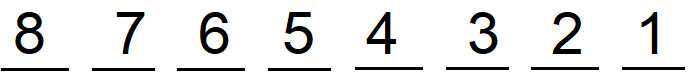
\includegraphics[width=0.4\textwidth]{slike/permutacija1.png}
    \end{figure}
    
    Odgovor: $ 8 \cdot 7 \cdot 6 \cdot \ldots \cdot 2 \cdot 1 = 40.320 $ možnosti.
    
    \didopomba{Kot zanimivost:} Koliko časa potrebujejo, da porabijo vse kombinacije, če skupaj obedujejo trikrat na dan? (13.440 dni $ \approx 37 $ let)

    \item Na koliko načinov lahko razporedimo 4 različne kroglice v vrsto? ($ 4 \cdot 3 \cdot 2 \cdot 1 = 24 $)
    
    \begin{figure}[h]
        \centering
        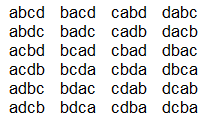
\includegraphics[width=0.3\textwidth]{slike/permutacija2.png}
    \end{figure}

\end{itemize}

\textcolor{red}{\textbf{Permutacija} = razporeditev $ n $ različnih elementov na $ n $ mest.}
Število permutacij $ n $ elementov običajno označimo z $ P_n $.

\didopomba{število elementov = število mest}
$$ P_n = n \cdot (n - 1) \cdot (n - 2) \cdot \ldots \cdot 2 \cdot 1 = n! $$
\didopomba{$ n! = $ ``n fakulteta'' oz. ``n faktorsko''. To je produkt vseh števil od 1 do $ n $.}

Dogovor: $ 0! = 1 $ \didopomba{pa lih paše iz $ n! = n \cdot (n - 1)! $}

\newpage

\vaje{
Vaja:
Na obisk prideta 2 Španca, 3 Nemci in 4 Slovenci. V kinu je v eni vrsti ravno 9 sedežev. \didopomba{pomoč s črticami in krogci, ki zajemajo isto narodnost. Naj čimveč sami predlagajo}
\begin{itemize}
    \item na koliko načinov se lahko usedejo v vrsto, brez omejitve? ($ 9! $)
    \item Na koliko načinov se lahko usedejo, če naj ljudje iste narodnosti sedijo skupaj? ($ 3! \cdot 2! \cdot 3 \cdot 4 $)
    \item Kaj pa, če morajo skupaj sedeti le Nemci, za ostalo pa ni važno? ($ 7! \cdot 3! $)
    \item Nemci sedijo na začetku vrste. ($ 3! \cdot 6! $)
    \item Španca sedita vsak na svojem koncu vrste ($ 2! \cdot 7! $)
    \item \didopomba{ZANIKANJE} Koliko je možnosti, da Slovenci ne sedijo vsi skupaj? (vse možnosti MINUS možnosti, da sedijo vsi skupaj $ = 9! - 4! \cdot 6! $)
    \item Slovenci sedijo na stolih s sodo številko ($ 4! \cdot 5! $)
\end{itemize}
Ostale vaje:
\begin{itemize}
    \item $ 6! - 4! = 6 \cdot 5 \cdot 4! - 4! = (30 - 1) \cdot 4 ! = 29 \cdot 24 = 696 $
    \item $ \frac{(n + 1)!}{(n - 3)!} = $ ? \didopomba{števec razpišeš na daljši del in pokrajšaš imenovalec}
    \item $ \frac{7!}{3!} = $ ?
    \item Upgrade motivacijske naloge: na koliko načinov se 8 oseb lahko usede za okroglo mizo? \didopomba{SLIKCA! Če se vsak premakne za eno mesto vstran, je razporeditev enaka, zato eno mesto fiksiramo za prvo osebo in ostale razporedimo na preostalih 8 mest ALI od vseh možnosti odstranimo premike za eno mesto}: $ 1 \cdot 8 \cdot 7 \cdot \ldots \cdot 2 \cdot 1 = \frac{9!}{9} = 8! $
\end{itemize}
}

\textcolor{red}{\textbf{Permutacije $ n $ elementov s ponavljanjem:}}

Imamo zeleno, modro in 3 rdeče kroglice, ki jih ne razlikujemo. Na koliko načinov jih lahko razporedimo v vrsto? \didopomba{Če jih razlikujemo, je odgovor $ 5! $, tako pa vrstni red rdečih med seboj ni pomemben, zato delimo s $ 3 ! \rightarrow 20 $}

\vaje{Še kakšen podoben primer, npr. permutacije črk besede ANANAS = $ \frac{6!}{3! \cdot 2!} = 60 $}

\end{priprava}